\documentclass[10pt, a4paper]{article}
\usepackage{fontspec}
\usepackage[top=1in, bottom=1in, left=1.1in, right=1.1in]{geometry}
\setlength{\headheight}{14.5pt}
\usepackage{xcolor}
\usepackage{hyperref}
\usepackage{graphicx}
\usepackage{microtype}
\usepackage{parskip}
\usepackage{setspace}
\usepackage{booktabs}
\usepackage{float}
\usepackage{caption}
\usepackage{fancyhdr}
\usepackage{titlesec}
\usepackage{enumitem}
\usepackage{amsmath, amssymb}

\setmainfont{TeX Gyre Termes}
\setsansfont{TeX Gyre Heros}
\setmonofont{TeX Gyre Cursor}

\hypersetup{colorlinks=true, linkcolor=black, urlcolor=black!70, citecolor=black}

\titleformat{\section}{\sffamily\Large\bfseries}{\thesection}{0.8em}{}
\titleformat{\subsection}{\sffamily\large\bfseries}{\thesubsection}{0.7em}{}

\pagestyle{fancy}
\fancyhf{}
\fancyhead[L]{\small\sffamily MNIST MLP report}
\fancyhead[R]{\small\sffamily\thepage}
\renewcommand{\headrulewidth}{0.4pt}
\fancypagestyle{plain}{\fancyhf{}\fancyfoot[C]{\small\sffamily\thepage}\renewcommand{\headrulewidth}{0pt}}

\captionsetup{font=small, labelfont=bf, labelsep=period, skip=8pt}
\setlist{nosep, leftmargin=1.5em}

\renewcommand{\topfraction}{0.9}\renewcommand{\bottomfraction}{0.9}\renewcommand{\textfraction}{0.1}\renewcommand{\floatpagefraction}{0.8}
\begin{document}
\setstretch{1.15}

\begin{center}
  {\sffamily\LARGE\bfseries A Three-Hidden-Layer MLP on MNIST}\\[0.6em]
  {\large Training, evaluation and error analysis}\\[0.3em]
  {\small\color{black!60} November 2026}
\end{center}
\vspace{1em}

\begin{abstract}\noindent
A plain fully connected network with three hidden layers ($784\to512\to256\to128\to10$, 567{,}434 parameters)
reaches \textbf{97.95\%} test accuracy on MNIST, with the training epoch selected on a held-out validation set and the test set used once. Training takes about 21 seconds on an Apple GPU.
This report documents the protocol, the data, the training curves, and where the remaining 205 errors come from.
\end{abstract}

\section{Introduction}

Handwritten digit recognition on MNIST is the standard first benchmark for neural classifiers, and a fully connected network is its simplest competitive baseline. This report evaluates such a baseline, a multilayer perceptron (MLP) with three hidden layers, and looks beyond a single accuracy number: the properties of the data, the training dynamics, per-class behaviour, and the failure cases. The result is a reference point against which regularised, augmented or convolutional models can later be compared.

\section{Method}\label{sec:method}

\textbf{Data.} The 60{,}000 MNIST training images are split at random (seed 0) into 55{,}000 for training and 5{,}000 for validation. The 10{,}000 test images are held out and used once, at the end (Section~\ref{sec:eda}). Pixels are scaled to $[0,1]$ and standardised with mean $0.1307$ and standard deviation $0.3081$. No augmentation.

\textbf{Model.} Each image is flattened to a 784-vector and passed through three ReLU hidden layers of width 512, 256 and 128, followed by a linear layer with 10 outputs (Table~\ref{tab:arch}).

\begin{table}[H]
  \centering
  \caption{Architecture and parameter count.}\label{tab:arch}
  \begin{tabular}{llrr}
    \toprule
    \textbf{Layer} & \textbf{Shape} & \textbf{Activation} & \textbf{Parameters} \\
    \midrule
    Hidden 1 & $784 \to 512$ & ReLU & 401{,}920 \\
    Hidden 2 & $512 \to 256$ & ReLU & 131{,}328 \\
    Hidden 3 & $256 \to 128$ & ReLU & 32{,}896 \\
    Output   & $128 \to 10$  & softmax (in the loss) & 1{,}290 \\
    \midrule
    \multicolumn{3}{l}{\textbf{Total}} & \textbf{567{,}434} \\
    \bottomrule
  \end{tabular}
\end{table}

\textbf{Optimisation.} Cross-entropy loss, Adam with learning rate $10^{-3}$, batch size 128, 10 epochs, seed 0, PyTorch on the Metal (MPS) backend. Validation loss and accuracy are logged after every epoch, and the checkpoint with the highest validation accuracy (ties broken by lower validation loss) is kept. The test set is evaluated exactly once, on that checkpoint.

\section{Data}\label{sec:eda}

MNIST is 70{,}000 grey-scale $28\times28$ scans of handwritten digits (60{,}000 train, 10{,}000 test; the training part is split 55{,}000/5{,}000 into train and validation, Section~\ref{sec:method}), stored as 8-bit pixels. Figure~\ref{fig:samples} shows twelve random training images per class. The writing styles vary a lot within a class: slanted and upright 1s, 7s with and without a crossbar, 4s with open and closed tops, thin and heavy strokes. Neighbouring classes already look easy to confuse (9 and 7, 5 and 3, 6 and 4), which anticipates the error analysis in Section~\ref{sec:errors}.

\begin{figure}[t]
  \centering
  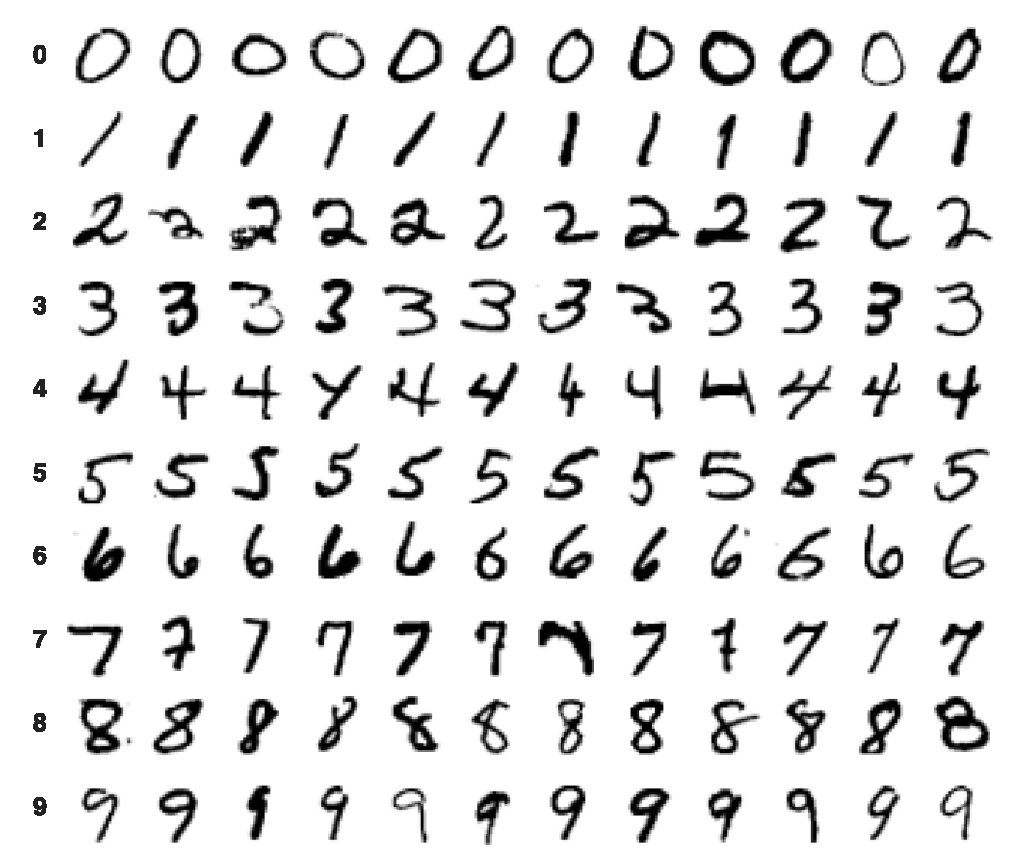
\includegraphics[width=0.6\textwidth]{eda_samples.pdf}
  \caption{Twelve random training images per digit.}\label{fig:samples}
\end{figure}

\textbf{Class balance.} The classes are close to balanced (Figure~\ref{fig:eda}, left): the training split ranges from 4{,}955 images for digit 5 (9.0\%) to 6{,}191 for digit 1 (11.3\%), the 5{,}000-image validation split from 466 (9.3\%) to 551 (11.0\%), and the test set follows similar proportions. A majority-class baseline would score 11.35\% on the test set, so plain accuracy is a fair metric and no class re-weighting is needed.

\textbf{Pixel statistics.} The images are sparse: 80.9\% of all pixels are exactly 0 and 7.4\% are saturated ($\geq250$), with little in between (Figure~\ref{fig:eda}, middle, log axis). The global mean is $0.1307$ and the standard deviation $0.3081$ on the $[0,1]$ scale, which are the constants used for input standardisation. Digits are centred by centre of mass in the $28\times28$ frame, and only 1.4\% of the training images have ink on the outermost pixel ring.

\textbf{Ink per digit.} The amount of ink differs strongly by class (Figure~\ref{fig:eda}, right). The median 1 has 57 units of ink against 135 for a 0, so a trivial ``how much ink'' feature already separates the 1 from the rest. Within every class the spread is wide, which reflects the stroke-width variation seen in Figure~\ref{fig:samples}.

\begin{figure}[H]
  \centering
  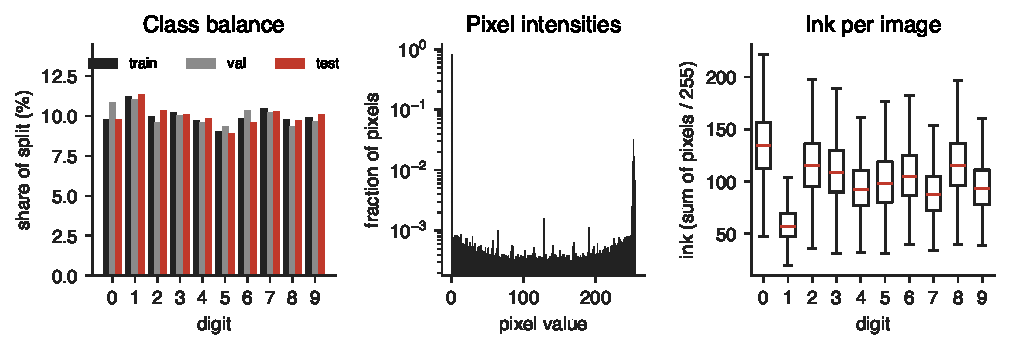
\includegraphics[width=\textwidth]{eda_stats.pdf}
  \caption{Class share per split, pixel-value histogram on a log axis (training split), and total ink per image by digit (box: quartiles, red: median).}\label{fig:eda}
\end{figure}

The class means (Figure~\ref{fig:mean}) are recognisable but blurry, and the 4/9 and 3/5/8 means overlap in the same regions. A model therefore has to rely on finer stroke detail than the average shape.

\begin{figure}[H]
  \centering
  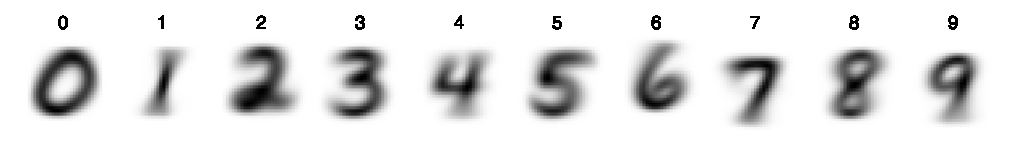
\includegraphics[width=\textwidth]{eda_mean.pdf}
  \caption{Mean training image per digit.}\label{fig:mean}
\end{figure}

\section{Training Results}

Figure~\ref{fig:curves} shows the two curves. Training loss falls monotonically from $0.269$ to $0.022$. Validation loss bottoms out at $0.082$ in epoch 4 and then drifts up to $0.104$, while validation accuracy fluctuates between 97.2\% and 97.6\% after epoch 3 and peaks at 97.62\% in epoch 7, the epoch that is kept (dashed line). The model overfits in loss terms (it grows more confident on its mistakes) but accuracy stays flat. Epochs 7 to 10 differ by at most 0.12 percentage points, six of the 5{,}000 validation images, so the exact choice of epoch is within noise.

\begin{figure}[H]
  \centering
  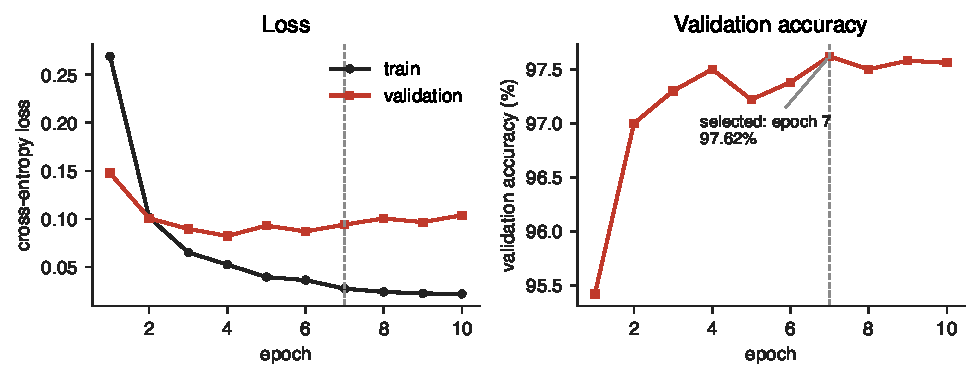
\includegraphics[width=\textwidth]{curves.pdf}
  \caption{Per-epoch training and validation loss (left) and validation accuracy (right). The dashed line marks the selected epoch.}\label{fig:curves}
\end{figure}

\begin{table}[H]
  \centering
  \caption{Per-epoch metrics on the training and validation splits. The selected epoch is in bold.}\label{tab:epochs}
  \begin{tabular}{rrrrr}
    \toprule
    \textbf{Epoch} & \textbf{Train loss} & \textbf{Val.\ loss} & \textbf{Val.\ acc.\ (\%)} & \textbf{Time (s)} \\
    \midrule
    1 & 0.2692 & 0.1476 & 95.42 & 2.6 \\
    2 & 0.1015 & 0.1006 & 97.00 & 2.1 \\
    3 & 0.0650 & 0.0895 & 97.30 & 2.0 \\
    4 & 0.0523 & 0.0822 & 97.50 & 2.0 \\
    5 & 0.0394 & 0.0929 & 97.22 & 2.0 \\
    6 & 0.0362 & 0.0869 & 97.38 & 2.0 \\
    \textbf{7} & \textbf{0.0272} & \textbf{0.0940} & \textbf{97.62} & \textbf{2.0} \\
    8 & 0.0239 & 0.1004 & 97.50 & 2.0 \\
    9 & 0.0223 & 0.0965 & 97.58 & 2.0 \\
    10 & 0.0217 & 0.1038 & 97.56 & 2.1 \\
    \bottomrule
  \end{tabular}
\end{table}

On the selected checkpoint the test accuracy is \textbf{97.95\%} (test loss $0.0763$), measured once. The standard error of an accuracy near 98\% is about 0.14 percentage points on the 10{,}000 test images and about 0.22 on the 5{,}000 validation images, so the 0.33-point gap between validation (97.62\%) and test accuracy is within sampling noise.

\section{Error Analysis}\label{sec:errors}

The selected model misclassifies 205 of 10{,}000 test images. Digit 7 has the lowest precision (0.966) and digit 6 the lowest recall (0.962) (Table~\ref{tab:class}); the cleanest classes are 0 and 1, with F1 above 0.987.

\begin{table}[H]
  \centering
  \caption{Per-class precision, recall and F1 on the test set.}\label{tab:class}
  \begin{tabular}{rrrrr}
    \toprule
    \textbf{Digit} & \textbf{Support} & \textbf{Precision} & \textbf{Recall} & \textbf{F1} \\
    \midrule
    0 &  980 & 0.9908 & 0.9857 & 0.9882 \\
    1 & 1135 & 0.9809 & 0.9947 & 0.9878 \\
    2 & 1032 & 0.9705 & 0.9884 & 0.9794 \\
    3 & 1010 & 0.9831 & 0.9762 & 0.9796 \\
    4 &  982 & 0.9767 & 0.9817 & 0.9792 \\
    5 &  892 & 0.9841 & 0.9731 & 0.9786 \\
    6 &  958 & 0.9957 & 0.9624 & 0.9788 \\
    7 & 1028 & 0.9655 & 0.9786 & 0.9720 \\
    8 &  974 & 0.9735 & 0.9805 & 0.9770 \\
    9 & 1009 & 0.9770 & 0.9703 & 0.9736 \\
    \bottomrule
  \end{tabular}
\end{table}

The confusion matrix (Figure~\ref{fig:cm}, diagonal left uncoloured so only mistakes stand out) shows that errors cluster on visually similar shapes.

\begin{figure}[H]
  \centering
  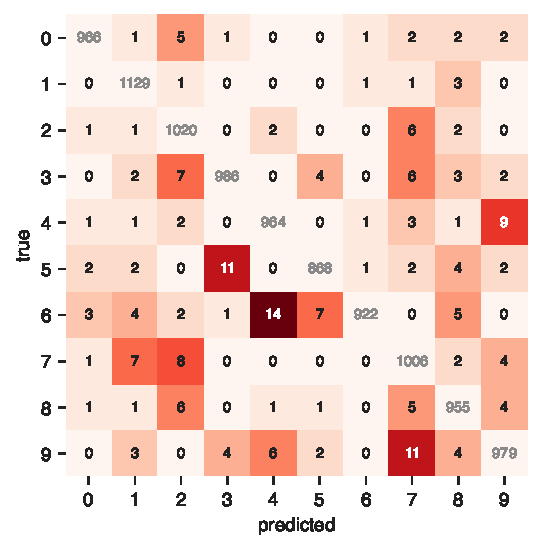
\includegraphics[width=0.5\textwidth]{confusion.pdf}
  \caption{Confusion matrix on the 10{,}000 test images (counts). Colour encodes off-diagonal counts only.}\label{fig:cm}
\end{figure}

Figure~\ref{fig:cex} shows the five most common confusions with the model's most confident examples of each (softmax probability in red). Many are genuinely ambiguous: a ``6'' with a flattened or open loop reads as a ``4'', a ``9'' with a broken loop or short slanted stem reads as a ``7'', a ``5'' with a flat top reads as a ``3'', a ``4'' with a closed top reads as a ``9'', and a ``7'' with a crossbar and curled foot reads as a ``2''.

\begin{figure}[H]
  \centering
  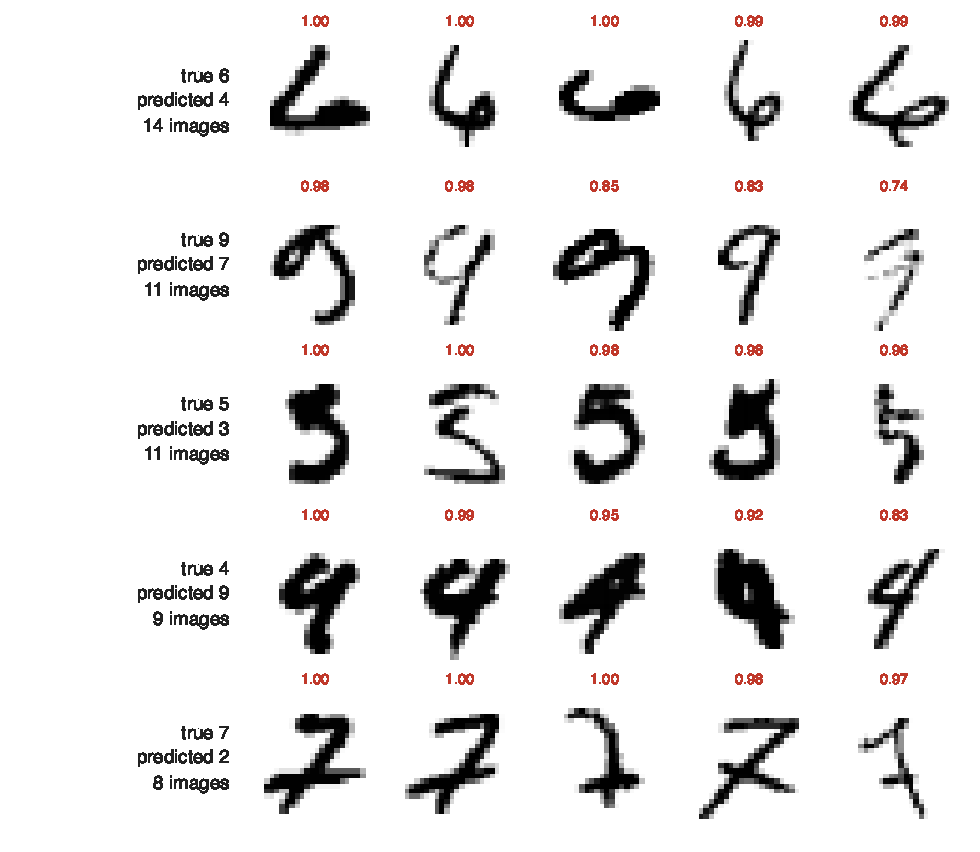
\includegraphics[width=0.92\textwidth]{confusion_examples.pdf}
  \caption{The five most common confusions, five most confident examples each. Left: true and predicted digit and the number of such errors in the test set.}\label{fig:cex}
\end{figure}

\subsection{Confident mistakes}

The examples in Figure~\ref{fig:cex} show that the network is often sure of itself when it is wrong, with several at probability $0.99$ or higher. Figure~\ref{fig:conf} compares the confidence of correct and wrong predictions: correct predictions average $0.993$, wrong ones $0.790$, so confidence is informative, but 80 of the 205 errors (39\%) still carry confidence above $0.9$. Flagging only low-confidence predictions would therefore miss about two in five mistakes.

\begin{figure}[H]
  \centering
  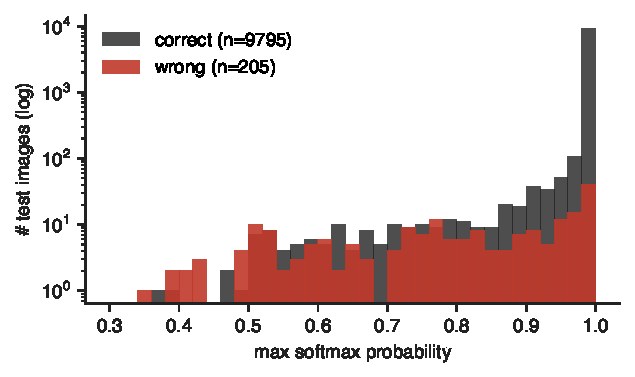
\includegraphics[width=0.65\textwidth]{confidence.pdf}
  \caption{Distribution of the winning softmax probability for correct and wrong predictions (log count axis).}\label{fig:conf}
\end{figure}

\section{Learned Features}

Each of the 512 first-layer units is a $28\times28$ weight map. Figure~\ref{fig:filters} shows the first 32. They are noisy and mostly non-local: some respond to stroke-like patterns and many to blobs at particular positions. This is typical for an MLP trained without convolutional structure or regularisation, which has to learn position-specific detectors rather than shared, translation-equivariant ones.

\begin{figure}[H]
  \centering
  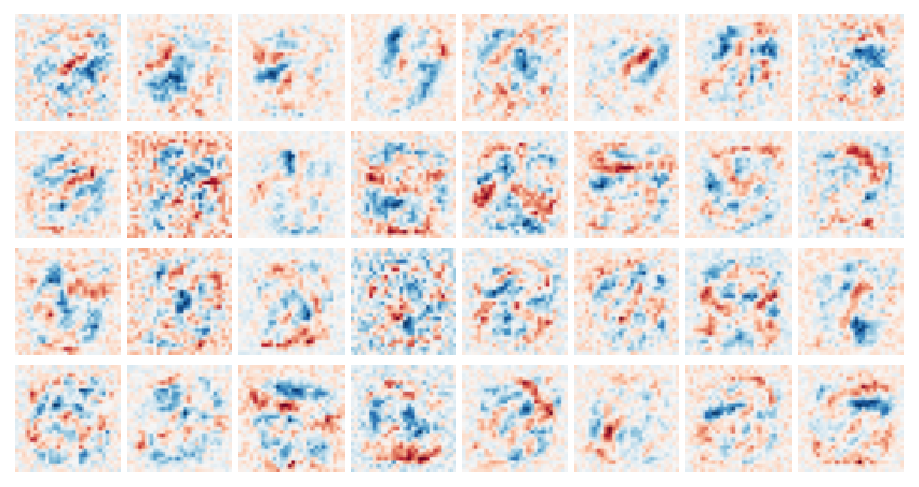
\includegraphics[width=0.72\textwidth]{filters.pdf}
  \caption{First 32 of 512 first-layer weight maps (red positive, blue negative, symmetric colour scale per map).}\label{fig:filters}
\end{figure}

\section{Conclusion}

A three-hidden-layer MLP with 567{,}434 parameters reaches 97.95\% test accuracy on MNIST after about 21 seconds of training, with the epoch (7 of 10) chosen on a 5{,}000-image validation split and the test set used once. Its 205 errors concentrate on visually ambiguous pairs (6/4, 9/7, 5/3, 4/9, 7/2), and 80 of them are made with confidence above 0.9, so output confidence alone is not a reliable error filter. The first-layer weights are noisy and position-specific, which is the expected signature of an MLP without convolutional structure.

\subsection*{Limitations}

\begin{itemize}
  \item The result is a single run (seed 0); run-to-run variation of a few tenths of a percent is expected.
  \item The validation split has only 5{,}000 images (standard error about 0.2 percentage points), so differences between nearby epochs or small configuration changes cannot be resolved with it.
  \item No regularisation, learning-rate schedule or augmentation was used, so the model is not tuned for accuracy.
\end{itemize}

\subsection*{Future Work}

\begin{enumerate}
  \item \textbf{Regularisation} (dropout or weight decay), since validation loss rises after epoch 4 while training loss keeps falling.
  \item \textbf{Learning-rate decay} (cosine or step) to settle into a better minimum in the last epochs.
  \item \textbf{Data augmentation} (small shifts and rotations), which targets the position-specific weights in Figure~\ref{fig:filters}.
  \item \textbf{Repeated seeds or $k$-fold cross-validation}, to report confidence intervals instead of a single run.
  \item \textbf{A convolutional model}, which typically exceeds 99\% on this dataset.
\end{enumerate}

\end{document}
